\section*{Appendix}

\subsection*{Description of the different variables}

The \textbf{response variable} is \textit{life.expectancy}.

The \textbf{explanatory variables} are the following:

Economic factors :
\begin{itemize}
	\item \textit{status}: is the country \textbf{developping} or \textbf{developped}.
	\item \textit{percentage.expenditure}: expenditure on health as percentage of gross domestic product (PIB in french) per capita (\%).
	\item \textit{total.expenditure}: general government expenditure on health as a percentage of total government expenditure (\%).
	\item \textit{gdp}: gross domestic product per capita (\$).
	\item \textit{income.composition.of.resources}: human development index (HDI) in terms of income composition of resources ($\in [0,1]$).
\end{itemize}

Social factors
\begin{itemize}
	\item \textit{population}: total population of the country.
	\item \textit{schooling}: number of years of schooling
\end{itemize}

Mortality factors : 
\begin{itemize}
	\item \textit{adult.mortality}: probability of dying between $15$ and $60$ years old (\textbf{very low}, \textbf{low}, \textbf{middle}, \textbf{high}, \textbf{very high}).
	\item \textit{under.five.deaths}: number of under five deaths per $1000$ population.
	\item \textit{infant.deaths}: number of infant deaths per $1000$ population.
	\item \textit{hiv.aids}: death per 1000 live births HIV/AIDS (between 0 and 4 years old).
	\item \textit{thinness.5.9.years}: prevalence of thinness among children for age $5$ to $9$ years old (\%).
	\item \textit{thinness.10.19.years}: prevalence of thinness among children and adolescents for age $10$ to $19$ years old (\%).
\end{itemize}

Immunization factors
\begin{itemize}
	\item \textit{hepatitis.b}: Hepatitis B immunization coverage among 1 year olds (\%).
	\item \textit{measles}: number of reported cases of measles per 1000 population.
	\item \textit{polio}: Polio immunization coverage among 1 year olds (\%).
	\item \textit{diphtheria}: Diphteria tetanus toxoid and pertussis (DPT3) immunization coverage among 1 year olds (\%)
\end{itemize}

Other factors
\begin{itemize}
	\item \textit{alcohol}: consumption of alcohol ($15$ years old or more) per capita (\textbf{in litres of pure alcohol}).
	\item \textit{bmi}: average BMI of entire population.
\end{itemize}

\subsection*{Histograms and boxplots of the explanatory variables}

% ECONOMIC

\begin{figure}[H]
	\centering
	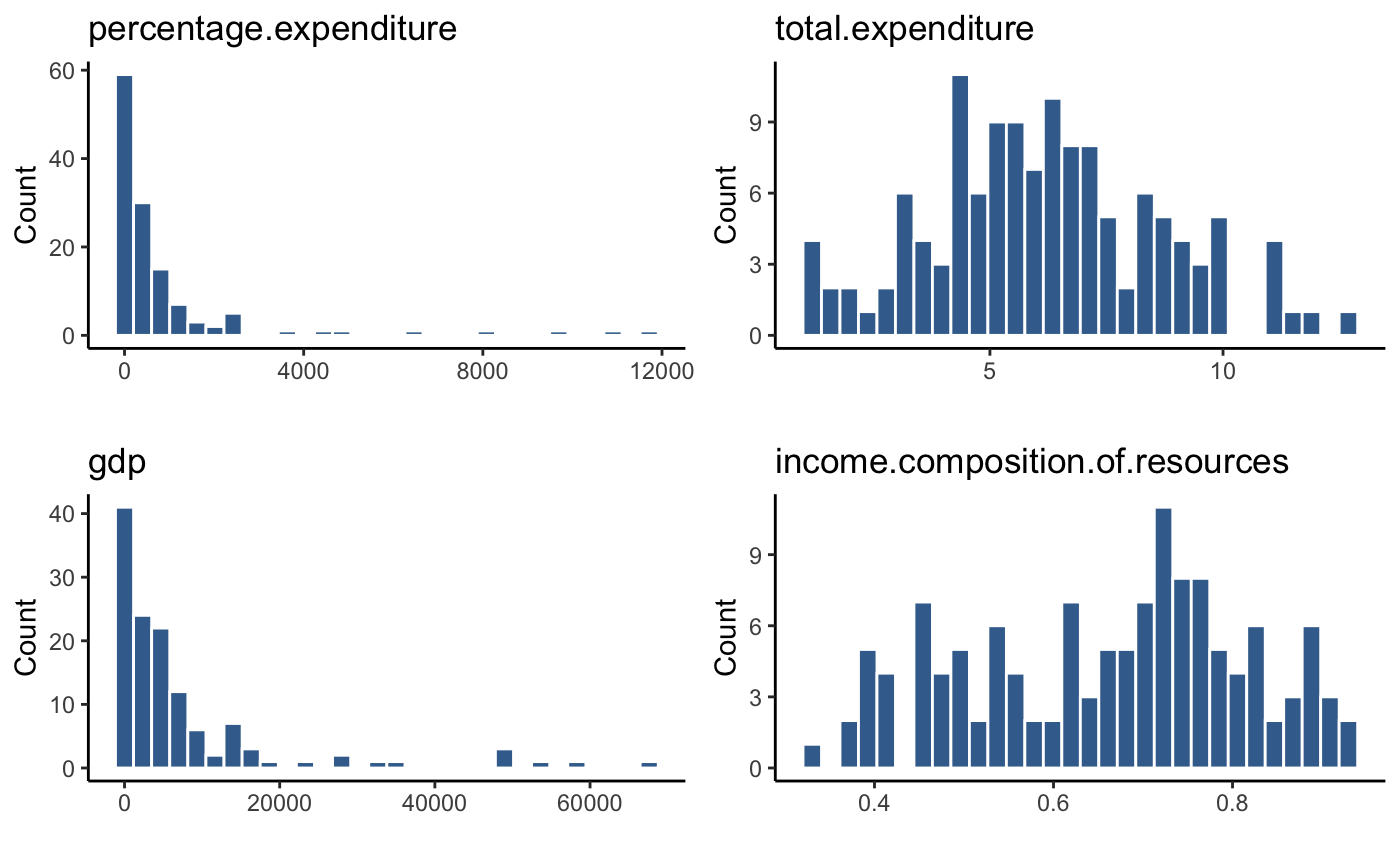
\includegraphics[width=0.5\textwidth]{figures/eda/histogram_economic_features.png}
	\caption{Histogram of economic features}
	\label{fig:histogram_economic_features}
\end{figure}

\begin{figure}[H]
	\centering
	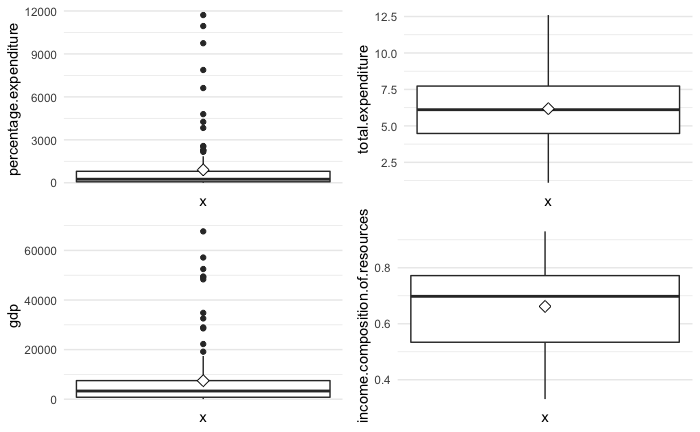
\includegraphics[width=0.5\textwidth]{figures/eda/boxplot_economic_features.png}
	\caption{Boxplot of economic features}
	\label{fig:boxplot_economic_features}
\end{figure}

% SOCIAL

\begin{figure}[H]
	\centering
	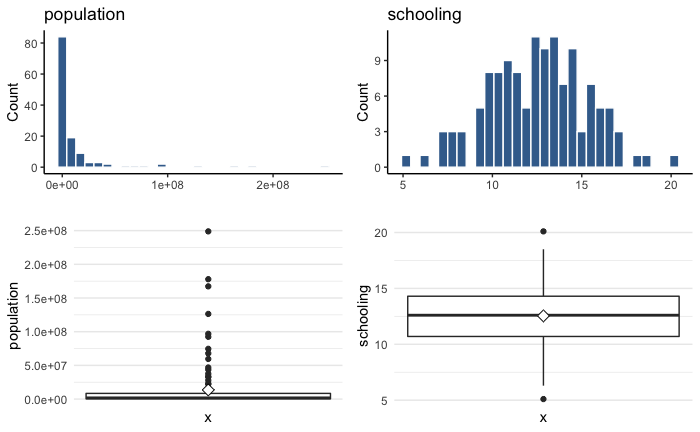
\includegraphics[width=0.5\textwidth]{figures/eda/histogram_boxplot_social_features.png}
	\caption{Histogram and boxplot of social features}
	\label{fig:histogram_boxplot_social_features}
\end{figure}

% MORTALITY

\begin{figure}[H]
	\centering
	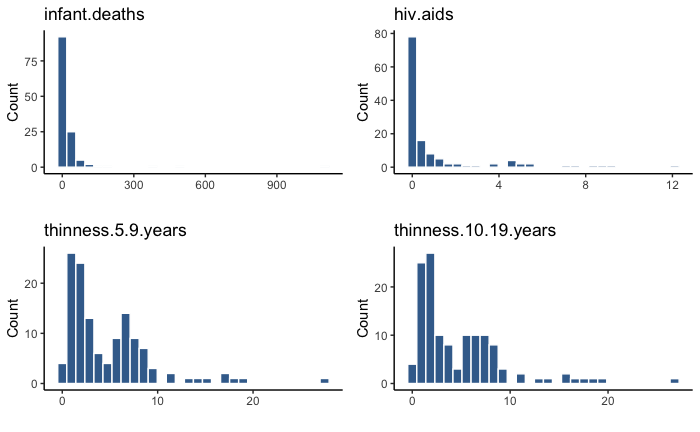
\includegraphics[width=0.5\textwidth]{figures/eda/histogram_mortality_features.png}
	\caption{Histogram of mortality features}
	\label{fig:histogram_mortality_features}
\end{figure}

\begin{figure}[H]
	\centering
	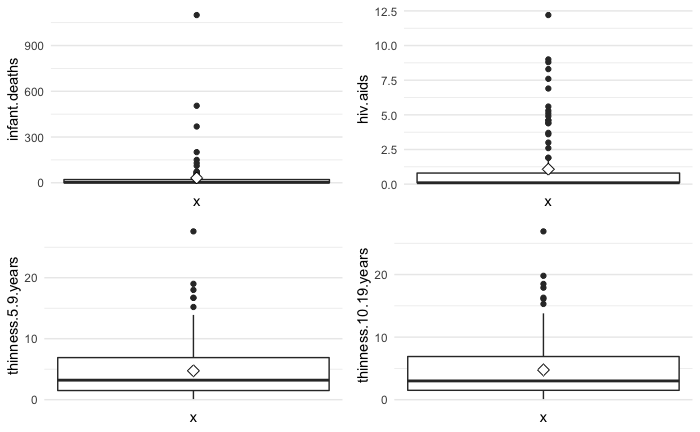
\includegraphics[width=0.5\textwidth]{figures/eda/boxplot_mortality_features.png}
	\caption{Boxplot of mortality features}
	\label{fig:boxplot_mortality_features}
\end{figure}

% HEALTH

\begin{figure}[H]
	\centering
	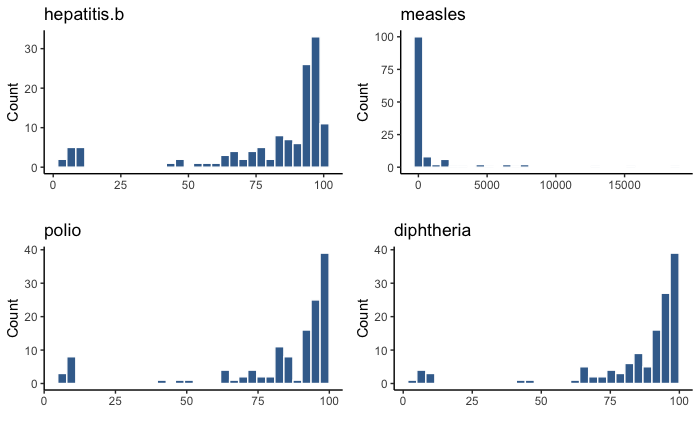
\includegraphics[width=0.5\textwidth]{figures/eda/histogram_health_features.png}
	\caption{Histogram of health features}
	\label{fig:histogram_health_features}
\end{figure}

\begin{figure}[H]
	\centering
	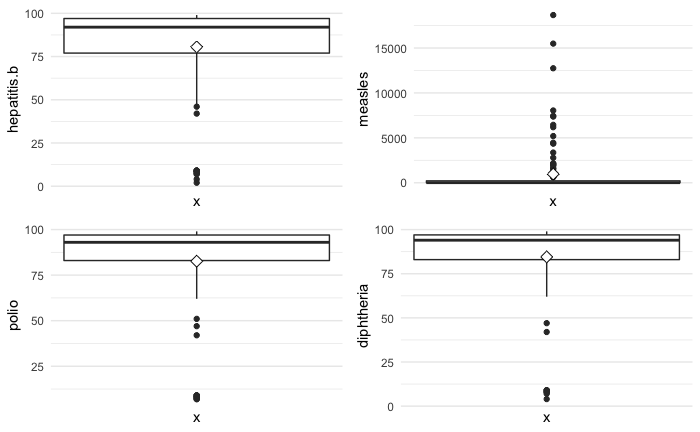
\includegraphics[width=0.5\textwidth]{figures/eda/boxplot_health_features.png}
	\caption{Boxplot of health features}
	\label{fig:boxplot_health_features}
\end{figure}

% OTHER

\begin{figure}[H]
	\centering
	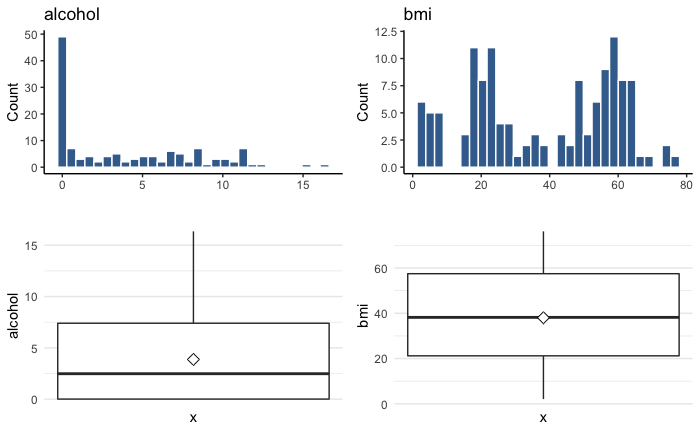
\includegraphics[width=0.5\textwidth]{figures/eda/histogram_boxplot_misc_features.png}
	\caption{Histogram and boxplot of misc features}
	\label{fig:histogram_boxplot_misc_features}
\end{figure}